\section{Kaggle Happywhale Challenge}
\addcontentsline{toc}{section}{Kaggle Happywhale Challenge}
\label{sec:kagglechallenge}

In the following chapter, we are explaining the Kaggle Happywhale challenge. This includes goal-setting and a comprehensive analysis of the dataset.

\subsection{Goal}
The Happywhale challenge is a research prediction competition, open to everybody with a Kaggle account. It's goal is to build a machine learning model which can reliably recognize individual whales and dolphins. The model should also be able to classify individuals it has never seen before as "new".
Such a model would save experts, who - up until now - have to analyse the images manually, a tremendous amount of work.


\subsection{Data}
The data \cite{kaggle} to be used for this challenge is split in to training and testing data. The training data consists of 51 thousand JPEG images of whales and dolphins. The training images are labeled with the according species and a unique individual identification string. The testing data consist of 28 unlabeled images containing some new whales and dolphins which are not present in the training data.\\
In total there are about 15 thousand different individuals and 30 different species. This data was manually curated by researchers from all over the world.

\begin{figure}[ht] 
        \centering 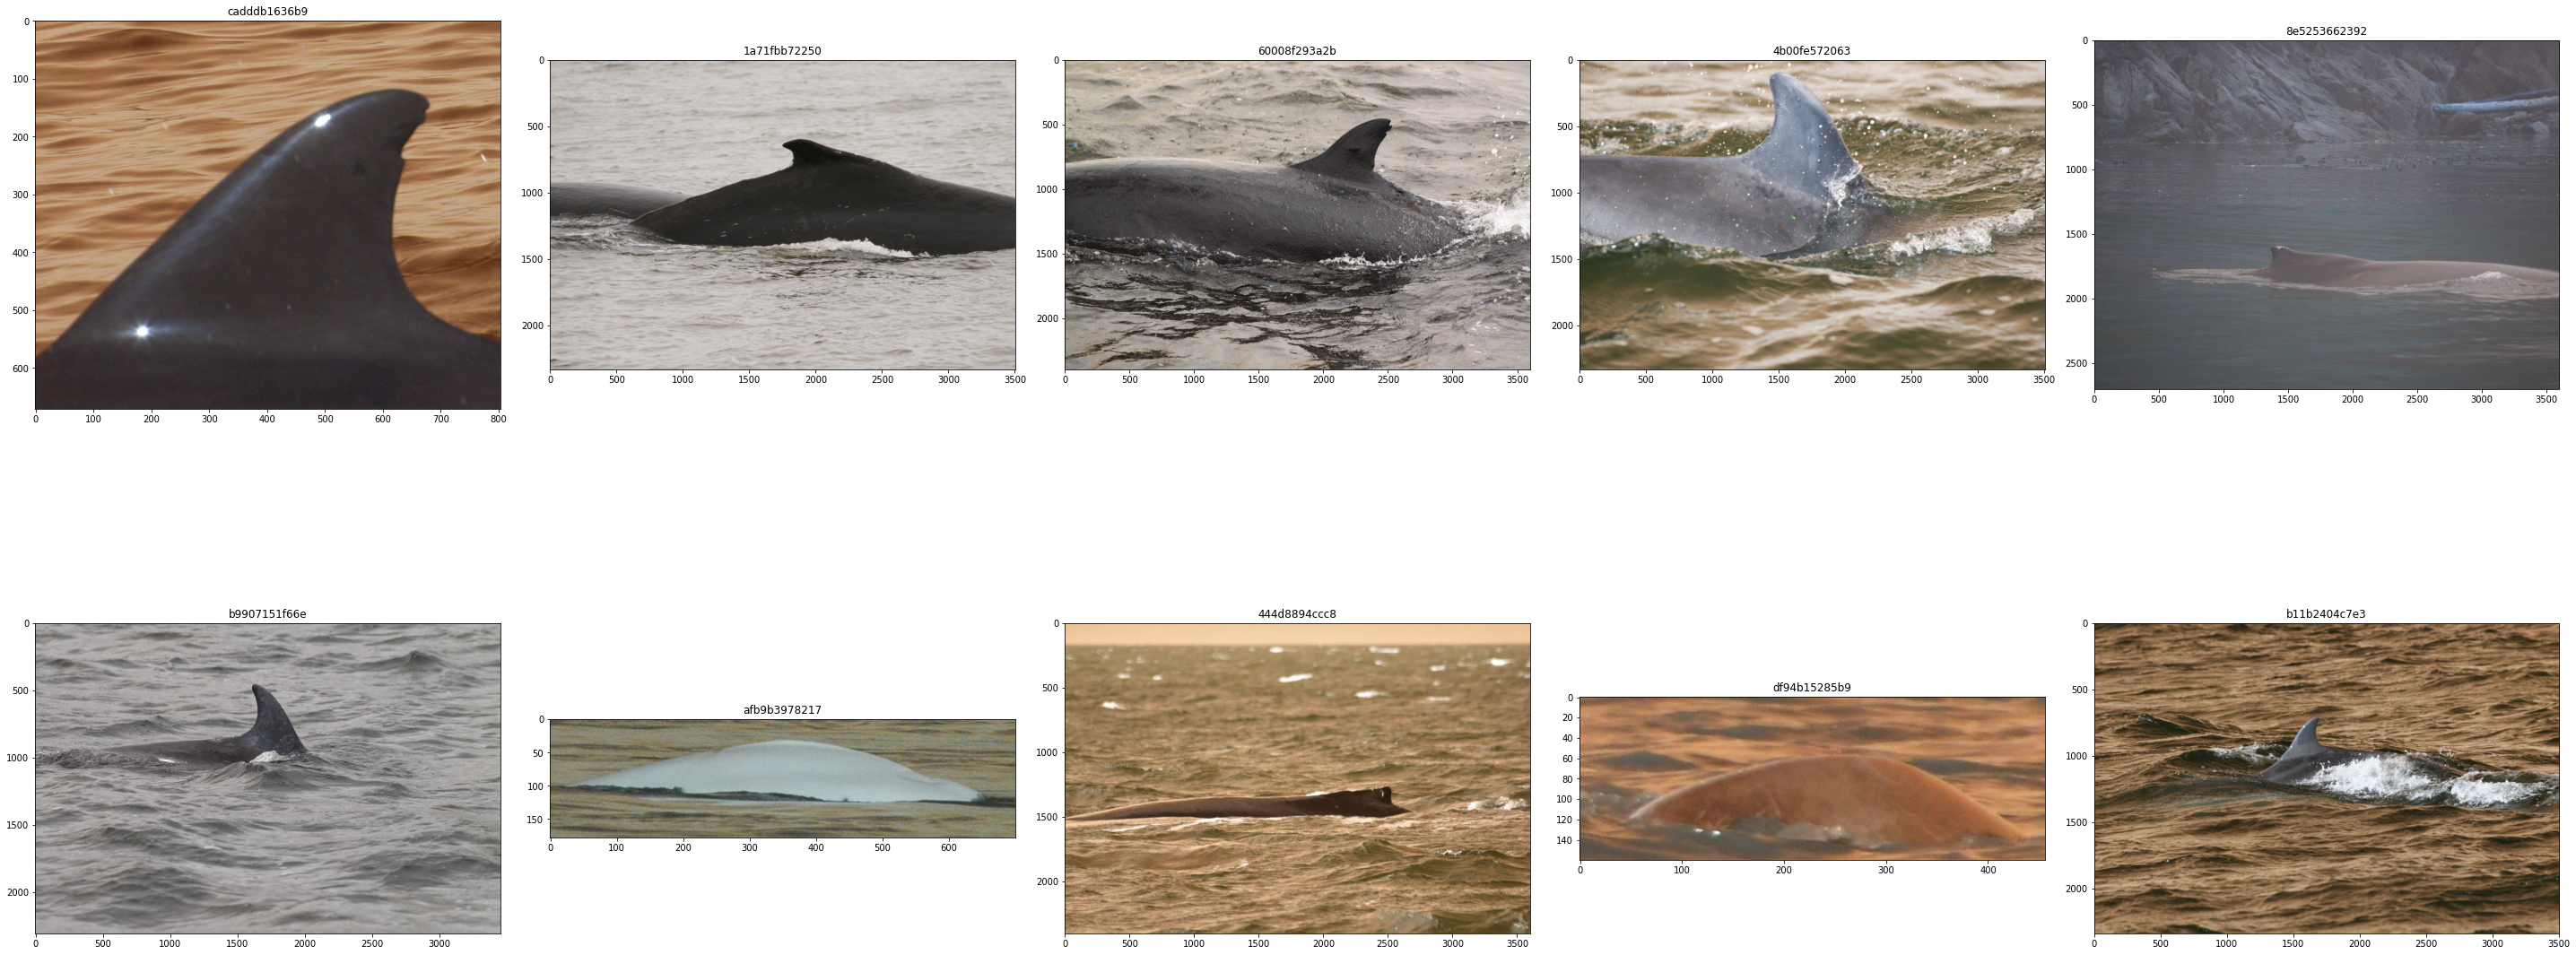
\includegraphics[width=1\columnwidth]{figures/original_images.png}
        \caption{\label{fig:original_images} Typical images from the data set.}
\end{figure}

\noindent With a median image shape of approximately (3000,1500), most images have high resolution. This makes unique patterns and markings of each individual identifiable by a neural network, even though most images only contain small parts of the marine animals such as dorsal fins and parts of the backs. \\
Some further analysis shows that 59\% of all individuals have only one image of themselves. They make out 18\% of all images in the data set.
5\% of all individuals have at least 10 images of themselves. These are 47\% of all images in the data set. \\
This is a large unbalance in number of images per individual and will make training of the network much harder.